%%%%%%%%%%%%%%%%%%%%%%%%%%%%
%%%%%%%%%%%%%%%%%%%%%%%%%%%%
\section{Consensus Methods} \label{sec:consensus}

Boostrap, jackknife and bayesian estimation naturally produce a forest of trees with the same species set. But different trees can also be estimated by using different methods or different sources of data. One way to summarize the forest is to \emph{project} it on a focal tree to compute support values (see section~\ref{sec:robustness}). Alternatively, one can bypass the focal tree altogether and combine all trees in the forest to get a single tree. That is the purpose of consensus trees methods.

%%%%%%%%%%%%%%%%%%%%%%%%%%%%
\subsection{Consensus Trees} \label{sec:consensus-tree}


\emph{Consensus trees} are trees that summarize a forest of trees with the same species set. We present here only the \emph{strict} consensus, the \emph{majority rule} consensus and the \emph{extended majority rule} consensus but there are many other consensus (see \citet{Bryant2003} for an extensive survey). The different notions are best understood on an example. Consider the forest featured in Figure~\ref{fig:consensus} with 40 copies of trees $T_1$, 48 of tree $T_2$ and 12 of tree $T_3$. Each tree is completely defined by the bipartitions it induces\footnote{or clades for for rooted trees}. For example, $T_1$ induces the partitions $AB|CDEF$, $ABCD|EF$ and $ABEF|CD$\footnote{or clades $AB$, $CD$, $EF$ and $CDEF$ if considered as rooted}, in addition to all trivial partitions $A|BCDEF$, $B|ACDEF$, etc not shown in the figure. Our three consensus methods scan the forest to build a list of all partitions occurring in the forest with their frequency of occurrence (middle column of Figure~\ref{fig:consensus}). They then select a subset of partitions according to some rules and build a consensus tree from that subset only.

\begin{figure}
 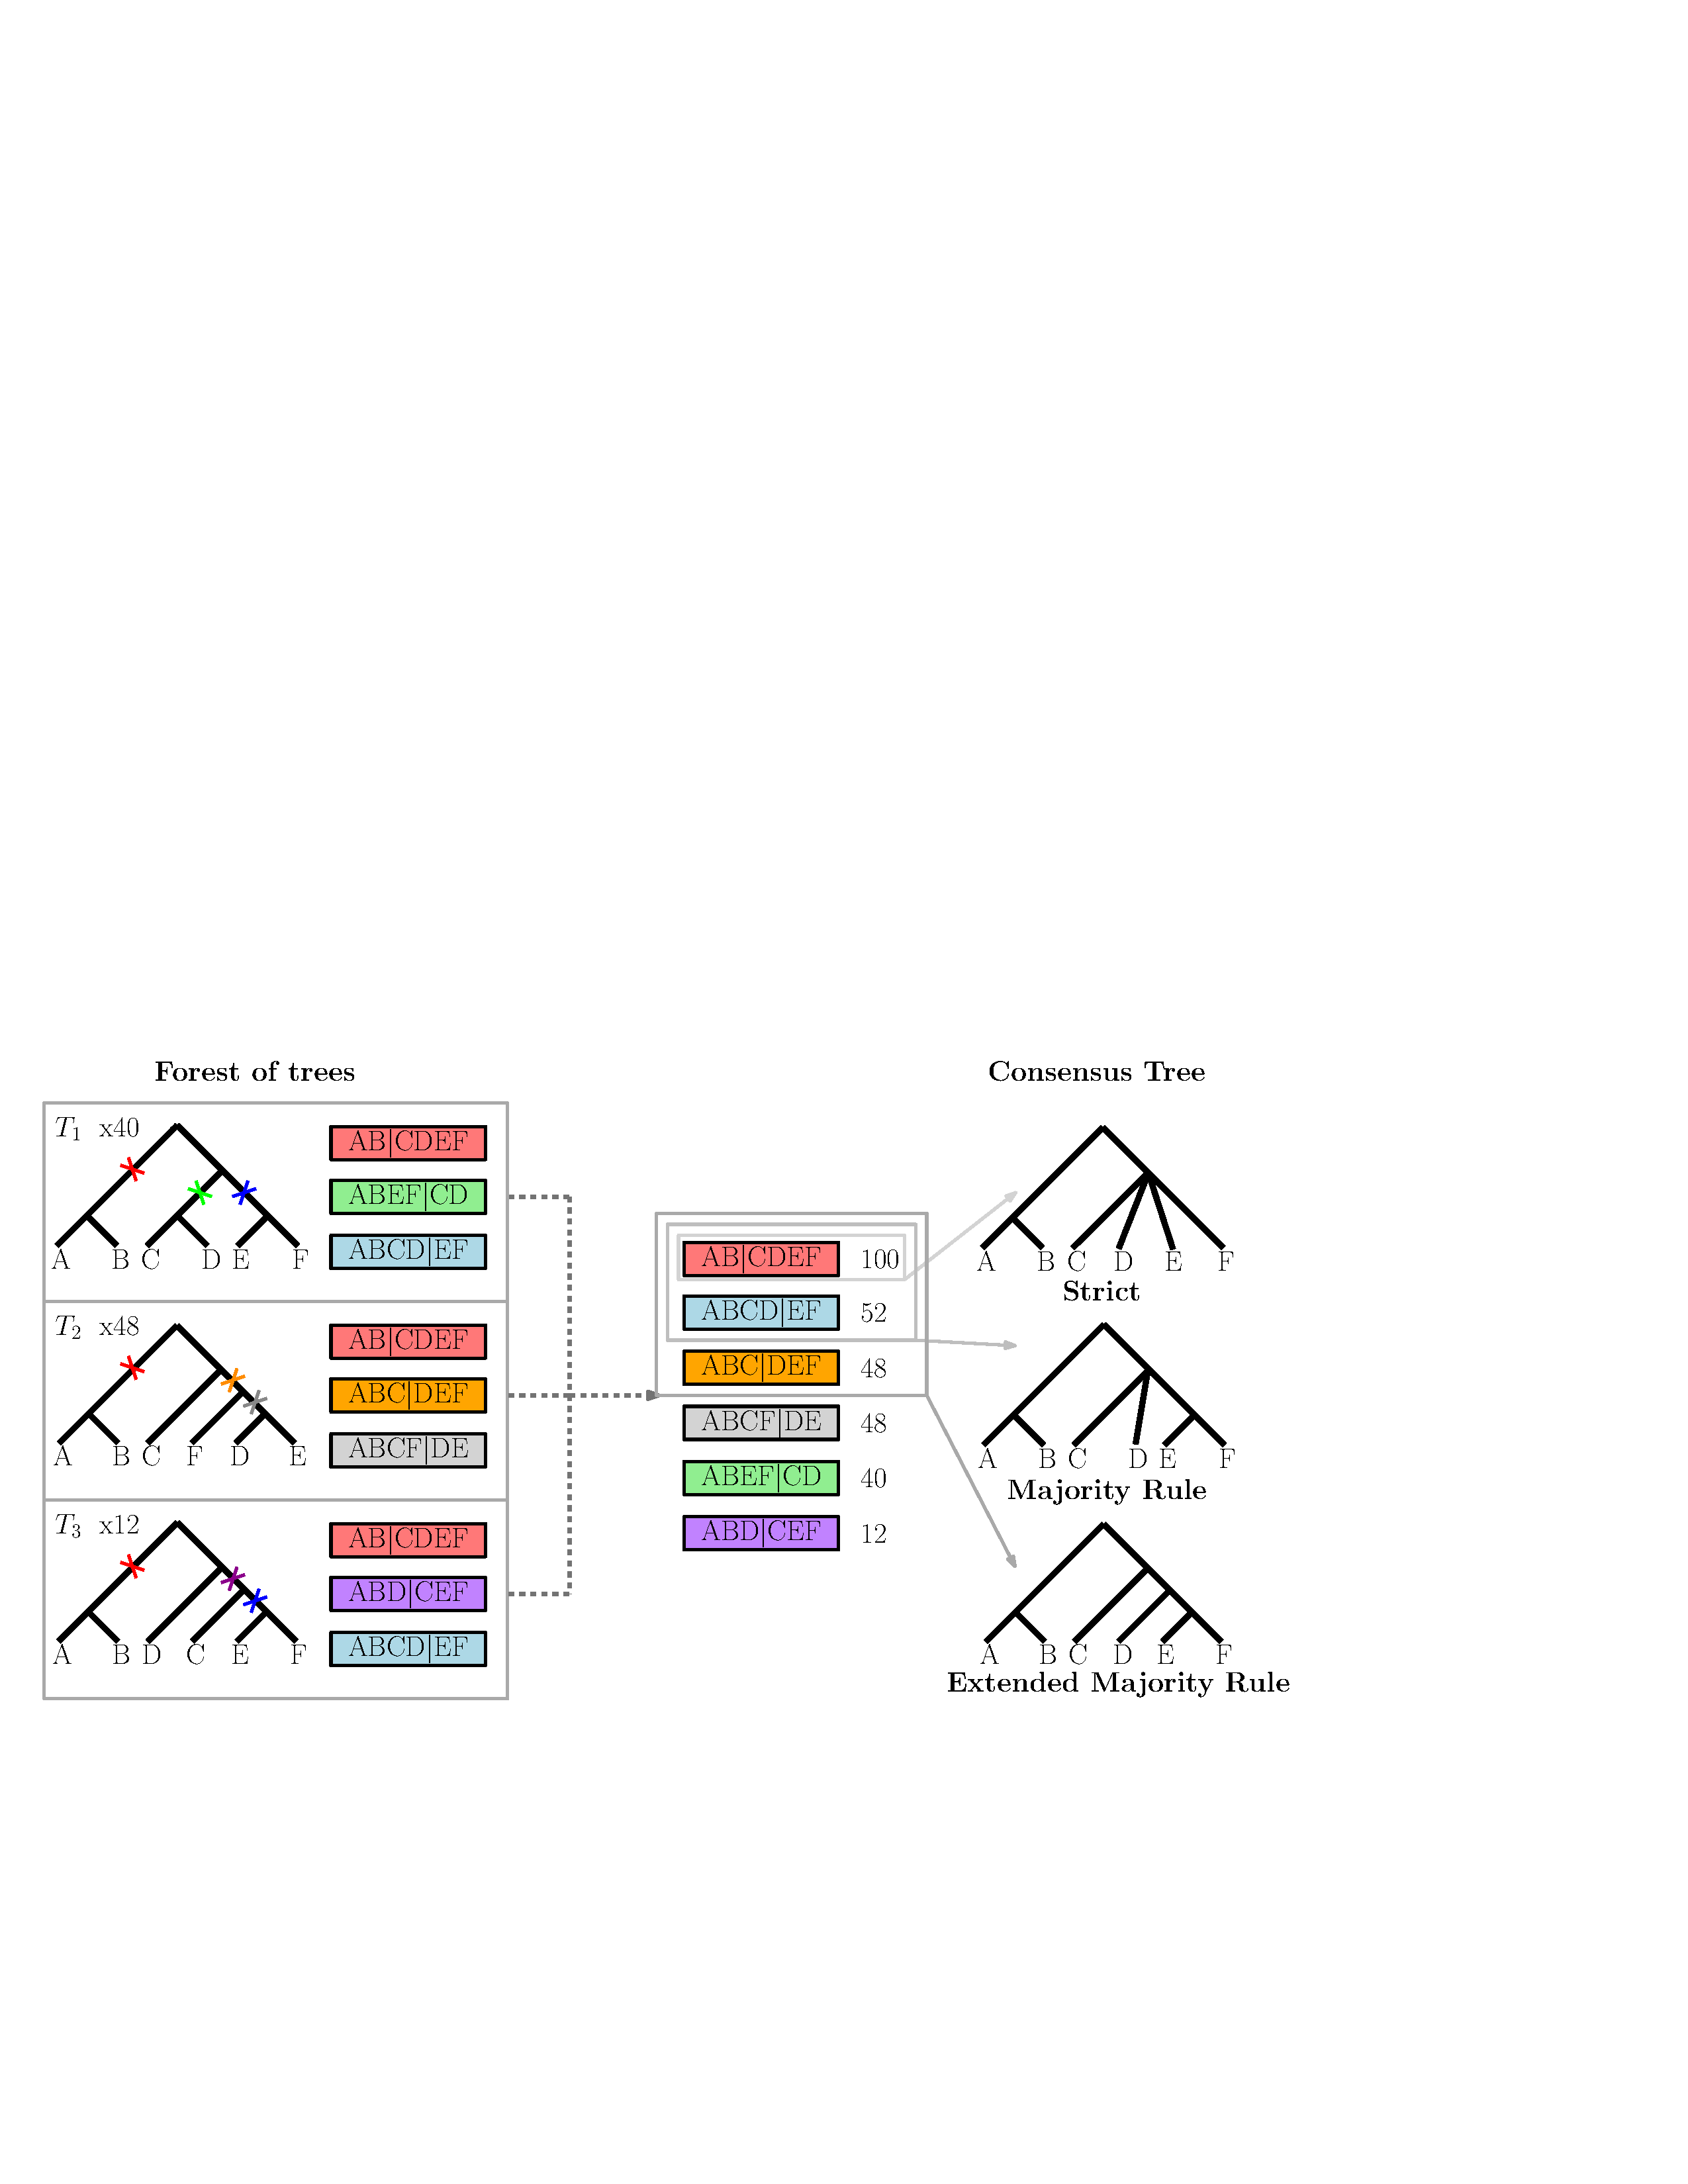
\includegraphics[width=0.9\linewidth]{Figs/consensus}
 \caption{Left: a forest of $100$ trees, corresponding to $3$ topologies. Each colored cross correspond to a non trivial bipartition. Middle: Set of all bipartitions, with their occurence frequencies, found in the forest. Right: Different consensus made up by increasing large sets of partitions.}
 \label{fig:consensus}
\end{figure}

%%%%%%%%%%%%%%%%%%%%%%%%%%%%
\subsubsection{Strict Consensus}

The \emph{strict consensus} tree \citep{Rohlf1982} only uses partitions that appear in \textbf{all} trees, \emph{i.e.} with a 100\% occurence frequency. The strict consensus is fully compatible with all trees in the forest. However, it is less resolved than any tree and usually too strict. In our example, $T_1$ and $T_2$ and $T_3$ only differ in the position of $D$: if we removed $D$ from all trees, they would be identical. We could therefore expect a branch separating $EF$ from $ABC$. However, the set $CDEF$ is completely unresolved in the strict consensus.

%%%%%%%%%%%%%%%%%%%%%%%%%%%%
\subsubsection{Majority-rule Consensus}

The \emph{majority-rule} consensus tree \citep{Margush1981} relaxes the condition that a bipartition must appear in all trees to be included in the consensus. Instead, it must only appear in \emph{most} trees, \emph{i.e.} have a occurrence frequency higher than 50\%. Although not obvious, all such partitions are pairwise-compatible and can be used to build a proper tree \citep{Buneman1971}. The majority-rule tree is more resolved than the strict consensus one but is not compatible with all trees in the forest. In our example, the partition $ABCD|EF$ seen in the majority-rule consensus is in conflict with the partition $ABCF|DE$ present in $T_2$.

%%%%%%%%%%%%%%%%%%%%%%%%%%%%
\subsubsection{Extended Majority-rule Consensus}

The \emph{extended majority-rule} consensus \citep{Felsenstein2005}, also called greedy consensus, relaxes the occurrence frequency condition even further. The consensus is build by sequentially adding partition one at a time, in decreasing order of occurrence and only if compatible with previously included partitions, until the tree is fully resolved or no more partitions can be added. Since all partitions with frequency higher than 50\% are compatible, they are part of the selection and the greedy consensus is thus a refinement of the majority-rule consensus. In our example, after including partitions $ABCD|EF$ and $AB|CDEF$, we can add either $ABC|DEF$ or $ABCF|DE$. The latter is in conflict with $ABCD|EF$ and thus not included whereas the former is compatible with both partitions and thus included. After addition of $ABC|DEF$, the greedy consensus is fully resolved. Note that the greedy consensus is different from all trees in the forest.

%%%%%%%%%%%%%%%%%%%%%%%%%%%%
\subsubsection{Branch Lengths in Consensus Trees}

The strict, majority-rule and extended majority-rule consensus trees only use \emph{toplogies} and produce consensus topologies. One way to add branch lengths to that consensus is to take, for each branch, its average length over trees where it is present. This is the approach used in MrBayes \citep{Ronquist2003} when building a consensus tree from the sample of posterior trees.

%%%%%%%%%%%%%%%%%%%%%%%%%%%%
\subsection{Distance-based Consensus} \label{sec:distance-based-consensus-tree}

The previous consensus methods are easy to understand and implement. Some also have a theoretical grounding that leads to generalizations. \citet{Barthelemy1986} showed that the majority-rule consensus is the \emph{center} of the forest in the sense that it minimizes the sum of Robinson-Foulds distances \citep{Robinson1979} to all trees in the forest. It is thus the forest \emph{median tree}. One could minimize total squared distance to all trees in the forest to find the \emph{mean tree}.

The Robinson-Foulds is but one of many distances between trees (see \citet{St.John2017} for an excellent review) and one can define other consensus similarly as the forest mean or median tree for some distance between tree. Although seducing, this approach suffered in the past from two shortcomings that severely limit its use. First, it was not obvious that the mean, or median, tree is well-defined or unique for some distances \citep{Billera2001}. Second, even when the mean was well-defined, there was no routine to compute it in practice. Recent progress in the field~\citep{Miller2015} have made it easier to compute sophisticated distances and use them to validate trees. % Computing the mean, variance and more general analyses of forest of trees based on tree distances is an active research field with many potential applications.
